
\subsection*{Experiment III: Auftriebskraft}\label{Experiment3}
\begin{figure}
    \subfigure{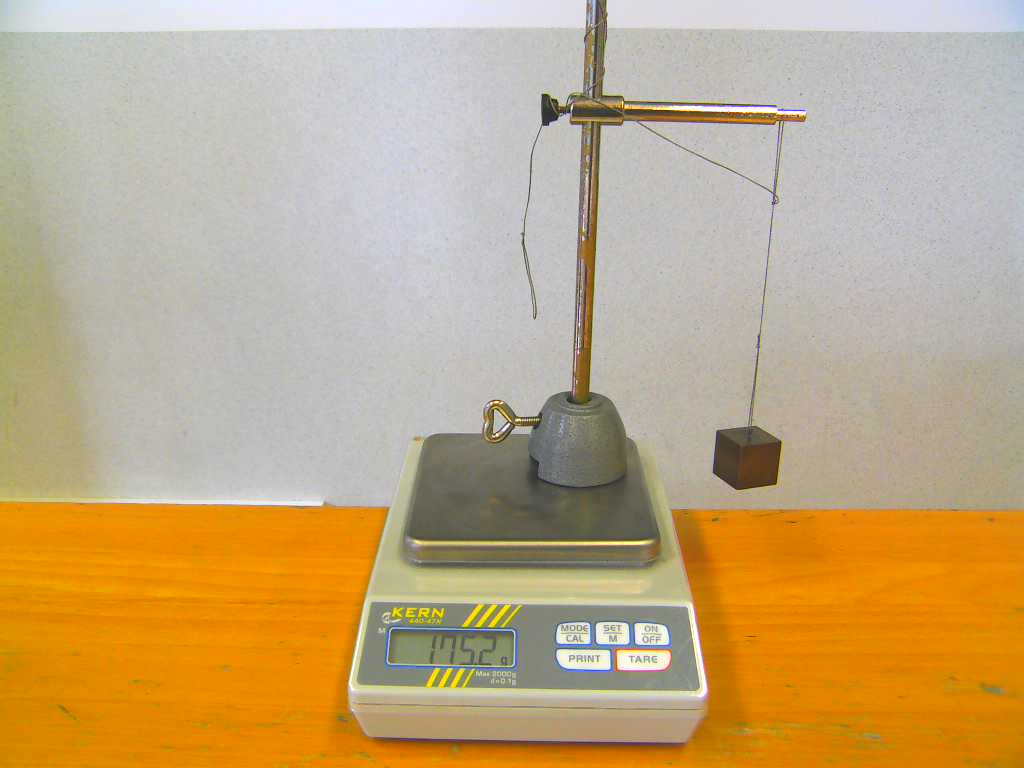
\includegraphics[width=0.49\textwidth]{\direxphyd/Luft.jpg}}
    \subfigure{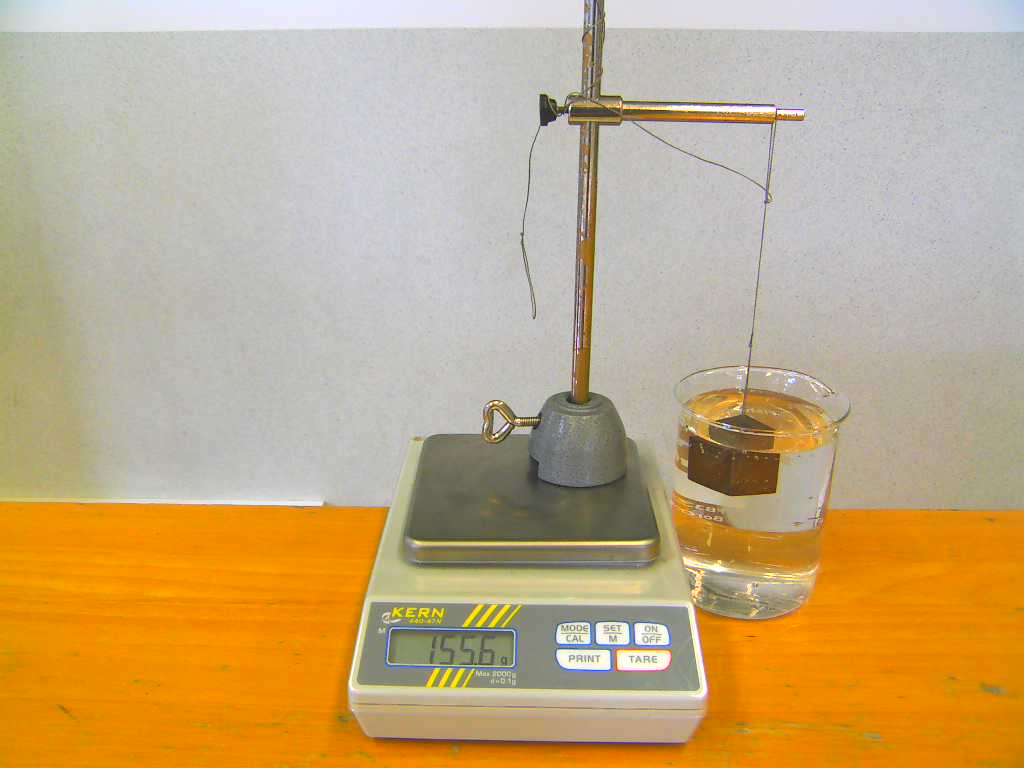
\includegraphics[width=0.49\textwidth]{./Wasser.jpg}}
\caption{Aufbau des Experiments zur Messung der Auftriebskraft. Auf der linken Seite sieht man das Wiegen in Luft, auf der rechten Seite wird
der selbe Metallwürfel in Wasser gewogen. Aus beiden Messungen zusammen lässt sich die Auftriebskraft bestimmen.}
\label{Fotoexperiment}
\end{figure} 

\begin{itemize}
	\item Glasgefäss (zum Beispiel Messbecher), Wasser
	\item elektronische Waage
	\item Stativ, dünner Bindfaden
	\item Würfel, Kugel (beides zum Aufhängen)
\end{itemize}

Dieses Demoexperiment kann wie folgt durchgeführt werden:



%\Spalten{0.5}%
%{\Bildeinbindencenter{Luft.jpg}{0.9}}%
%{0.5}%
%{\Bildeinbindencenter{Wasser.jpg}{0.9}}%


\begin{itemize}
	\item Wiegen des Würfels in Luft (siehe Abbildung \ref{Fotoexperiment}).
	\item Einhängen des Würfels in Wasser und erneutes Wiegen des Würfels.
	\item Bestimmen der Auftriebskraft (siehe Wandtafelskizze I).
	\item Verändern der Eintauchtiefe ohne Änderung der Auftriebskraft.
	\item Messen der Geometrie des Würfels (Kantenlänge).
	\item Berechnen der Auftriebskraft mit Hilfe des Schweredrucks der Flüssigkeit (Wandtafelskizze II)
\end{itemize}

